\documentclass[norsk,a4paper,12pt]{article}
\usepackage[T1]{fontenc} %for å bruke æøå
\usepackage[utf8]{inputenc}
\usepackage{graphicx} %for å inkludere grafikk
\usepackage{verbatim} %for å inkludere filer med tegn LaTeX ikke liker
\usepackage{amsfonts}
%\usepackage[framed]{mcode} %for å få inn matlabkode
\usepackage{listings}
\usepackage[margin=1.2cm]{caption} % skalere figur text
\usepackage{subfigure}

\bibliographystyle{plain}
\usepackage{parskip}
\usepackage{babel, textcomp, color, amsmath, amssymb, tikz, subfig, float}
\renewcommand{\captionfont}{\sffamily\small} 
\renewcommand{\captionlabelfont}{\bf} 
\fboxsep=0mm % ramme inn bilder


\title{FYS3150 - Project 1}
\author{Steffen Brask}
\date{\today}


\begin{document}

\maketitle

%\begin{center}
%Skrive noe smart her? GIT link?
%\end{center}


\newpage


\section*{Project 1}

The goal of this project is to solve the one-dimensional Poisson equation with Dirichlet bound-
ary conditions.

\subsection*{part a)}

the equation we are to solve has the form:
\begin{equation}
 \-u''(x) = f(x), \hspace{0.5cm} x\in(0,1), \hspace{0.5cm} u(0) = u(1) = 0.
\end{equation}
we can approximate the second derivative of a function with discrete values like this:
\begin{equation}
 -\frac{v_{i+1}+v_{i-1}-2v_i}{h^2} = f_i  \hspace{0.5cm} \mathrm{for} \hspace{0.1cm} i=1,\dots, n.
\end{equation}
Where $f_i=f(x_i)$, and $x_i$ is the discrete values of x defined as $x_i=ih$ where $h=1/(n+1)$.  \newline

If we now assume that we can solve this problem as a set of linear equations on the form:
\begin{equation}
 {\bf A}{\bf v} = \tilde{{\bf b}}.
\end{equation}
Where ${\bf A}$ is an $n\times n$  tridiagonal matrix, and $\tilde{b}_i=h^2f_i$. We now take a wild guess on the form 
of ${\bf A}$, because we know where we want to end up, so let ${\bf A}$ be:
\begin{equation}
    {\bf A} = \left(\begin{array}{cccccc}
                           2& -1& 0 &\dots   & \dots &0 \\
                           -1 & 2 & -1 &0 &\dots &\dots \\
                           0&-1 &2 & -1 & 0 & \dots \\
                           & \dots   & \dots &\dots   &\dots & \dots \\
                           0&\dots   &  &-1 &2& -1 \\
                           0&\dots    &  & 0  &-1 & 2 \\
                      \end{array} \right)
\end{equation}

Scince ${\bf v} = [v_1, v_2, ..., v_n]$, we can see here that:
\begin{equation}
    {\bf A}{\bf v} = \left(\begin{array}{cccccc}
                           2v_i& -1v_{i+1}& 0 &\dots   & \dots &0 \\
                           -1v_i & 2v_{i+1} & -1v_{i+2} &0 &\dots &\dots \\
                           0&-1v_{i+1} &2v_{i+2} & -1v_{i+3} & 0 & \dots \\
                           & \dots   & \dots &\dots   &\dots & \dots \\
                           0&\dots   &  &-1v_{n-2} &2v_{n-1}& -1v_n \\
                           0&\dots    &  & 0  &-1v_{n-1} & 2v_{n} \\
                      \end{array} \right)
\end{equation}

This gives for all the rows exept the first and last that the equation${\bf A}{\bf v} = \tilde{{\bf b}}$ gields
$\tilde{{\bf b_i}} = -v_{i-1} + 2v_{i} - v_{i+1}$, and scince $\tilde{b}_i=h^2f_i$, we therefore end up with the equation:
\begin{equation}
 -\frac{v_{i+1}+v_{i-1}-2v_i}{h^2} = f_i
\end{equation}

This is the base we are going to build our algorithm on. Be ware though that the first and last row is a little different.
But this is fine for our case scince we are solving the equation with $u(0) = u(1) = 0$

\subsection*{part b)}

We now need to outline the algorithm. The above tridiagonal system can be written as $a_iv_{i-1}+b_iv_i+c_iv_{i+1} = \tilde{b}_i$.
where $a_i = c_i = -1, and b = 2$. This system can be solved in two steps. (i) A forward substitution, and (ii) a backward substitution. \newline

(i)\newline
This step is all about making all the $c_i = 0$. To ensure $c_2 = 0$ we can subtract rowII from rowI times a constant. So:
$rowII - x*rowI$ for $c_2$ this gives an equation $c_2 = b_1*x \Rightarrow x = \frac{c_2}{b_2}$, with this constant $c_2 = 0$
and we have to apply this to the rest of the row: $b_2' = b_2 - a_1\frac{c_2}{b_1}$, and $u_2' = u_2 - u_1\frac{c_2}{b_1}$.
We now continue the procedure on rowIII: $x = \frac{c_3}{b_2'} \Rightarrow b_3' = b_3 - a_2\frac{c_3}{b_2'}$ and $u_3' = u_3 - u_2'\frac{c_3}{b_2'}$
And we now see the system, for each turn we ned to calculate the constant $x$, to get $b_i'$, which gives us $u_i'$. \newline

(ii)\newline
The next step is to make the diagonal = 1 (the $b_i =1$), and all the $a_i = 0$ to do this we use the same logic as step (i)
backwards $row(n-1) - x*row(n)$, this gives a constant $x = \frac{a_{n}}{b'_{n+1}}$, but we want to make $b'_{n+1} = 1$, and because
of this the tha constant $x = a_n$ and the whole bacwards substitution simplifies to $u''_n = u'_n - a_n*u_{n+1}$, and 
all we need to do now is to force the $n = 0$, and $n = n+1$ to be $0$ and let $n = n+2$ so we get the endpoints. My Main.cpp file
is added at the end of the PDF. i ran it with n= 10, 100, 1000 and here are the plots:

\begin{figure}[H]
  \begin{center}
    \subfigure[N = 10]{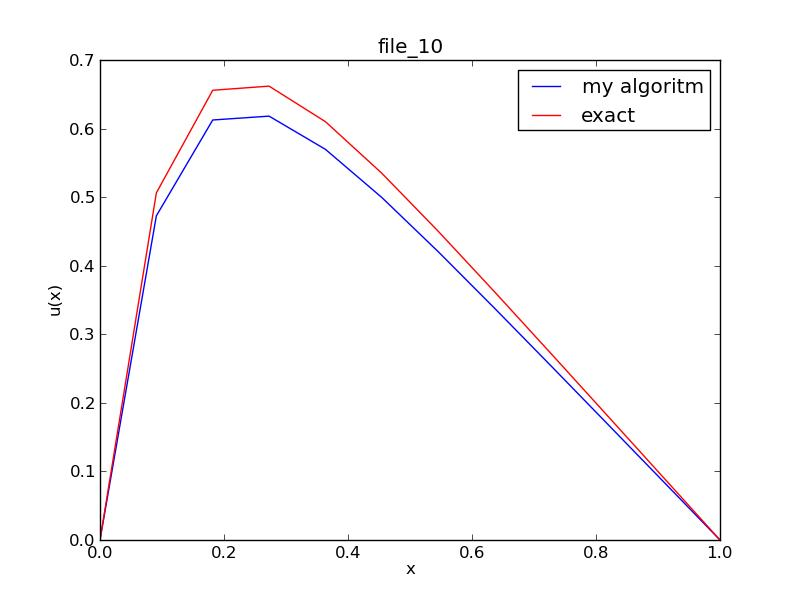
\includegraphics[scale=0.2]{plot_N_file_10.jpg}}
    \subfigure[N = 100]{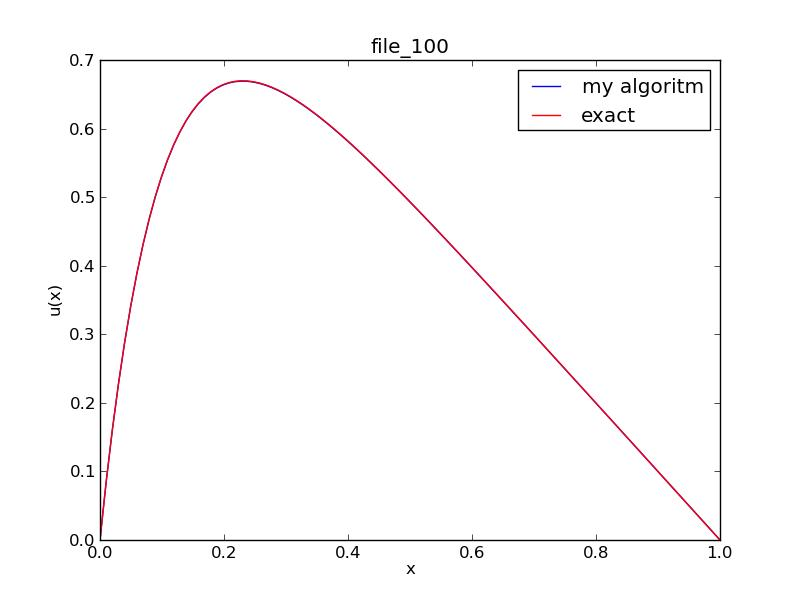
\includegraphics[scale=0.2]{plot_N_file_100.jpg}} \\
    \subfigure[N = 1000]{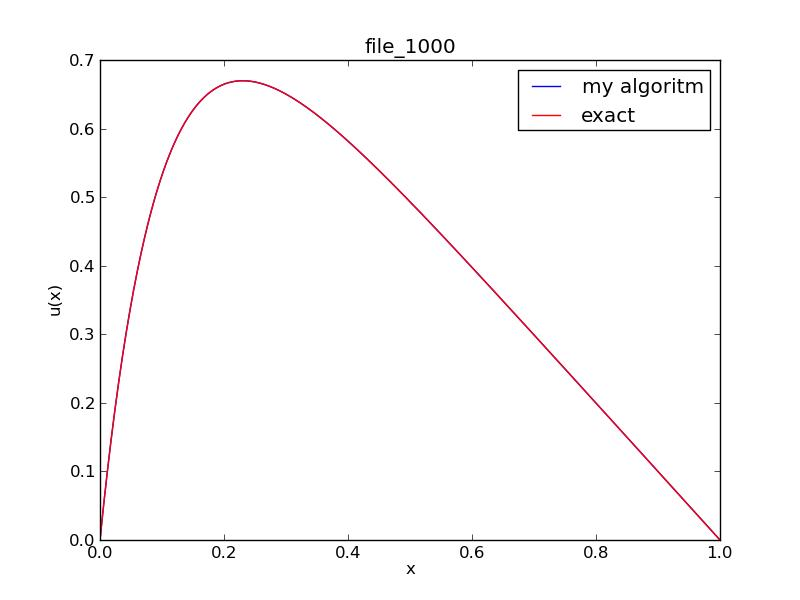
\includegraphics[scale=0.2]{plot_N_file_1000.jpg}}
  \end{center}
  \caption{\textit{plot of my algorithm vs exact analytical solution for different resolutions}}
  \label{fig:edge}
\end{figure}

We can see here that we lose precicion for n = 10, but for n = 100, and n = 1000 we get good aproximations.

\subsection*{part c)}

In this part we are going to compute the relative error in the algoritm for different values of n. We compute the relative error 
with the formula 
\begin{equation}
\epsilon_i=log_{10}\left(\left|\frac{v_i-u_i}
             {u_i}\right|\right),
\end{equation}

This is easily done by storing the data in a file and plotting in python. (Python script is added at the end). So lets look at some
plots!
\begin{figure}[H]
  \begin{center}
    \subfigure[N = 10]{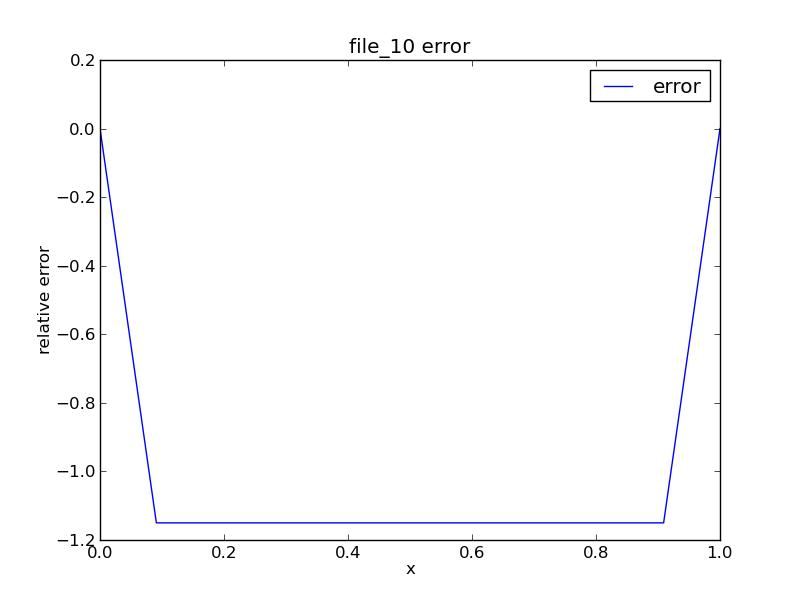
\includegraphics[scale=0.2]{error_n_10.jpg}}
    \subfigure[N = 100]{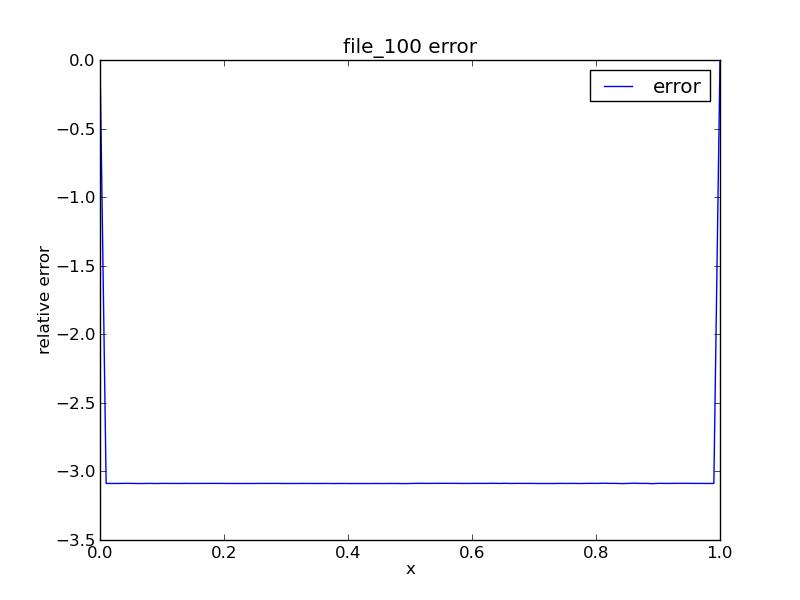
\includegraphics[scale=0.2]{error_n_100.jpg}} \\
    \subfigure[N = 1000]{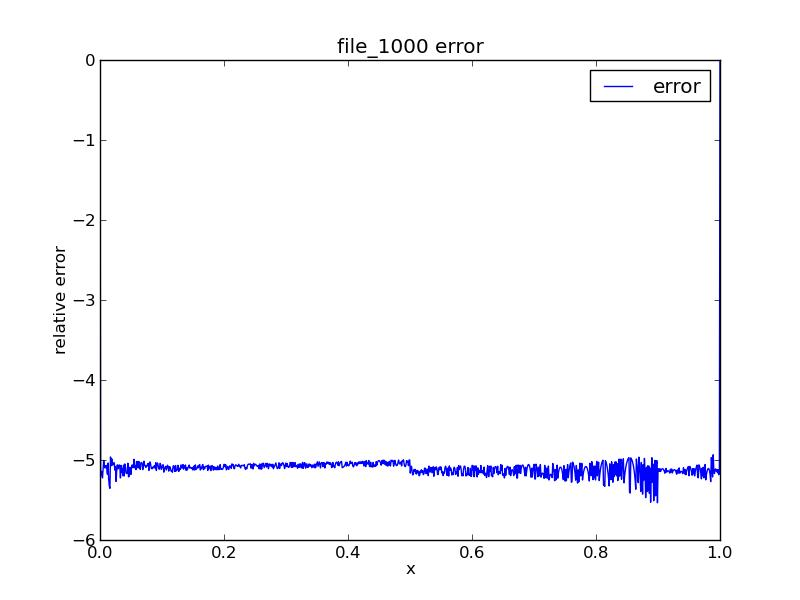
\includegraphics[scale=0.2]{error_n_1000.jpg}}
    \subfigure[N = 10000]{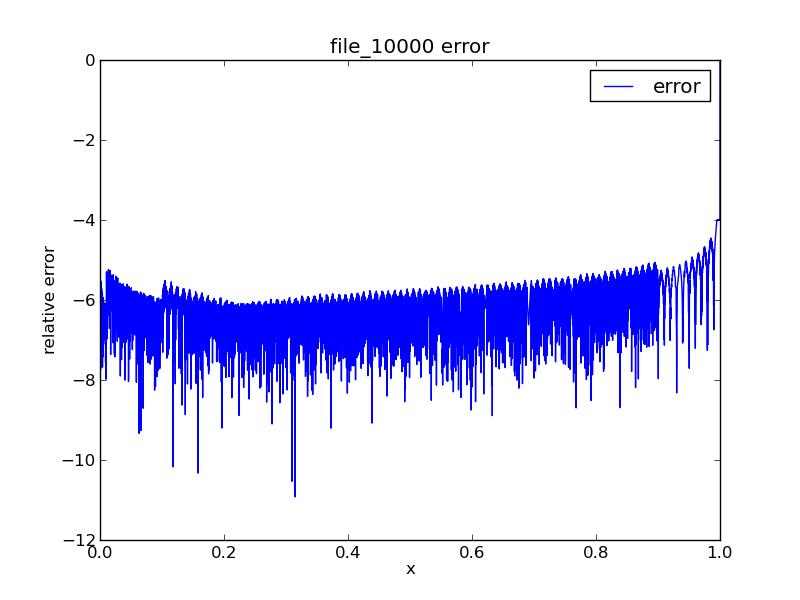
\includegraphics[scale=0.2]{error_n_10000.jpg}}
  \end{center}
  \caption{\textit{plot of my relative error for discrete values of x}}
  \label{fig:edge}
\end{figure}
I decided to add the plot of the error for each $\epsilon_i$ This is because i found them interesting. I would ecpect the error 
to increase gradually, but that is not the case. It seems to fluctuate for n = 1000, and n = 10000. I can not explain this.
I tried to check for n = 100000, but then i got a memory problem. 

\begin{figure}[H]
  \begin{center}
    \subfigure[N = 10]{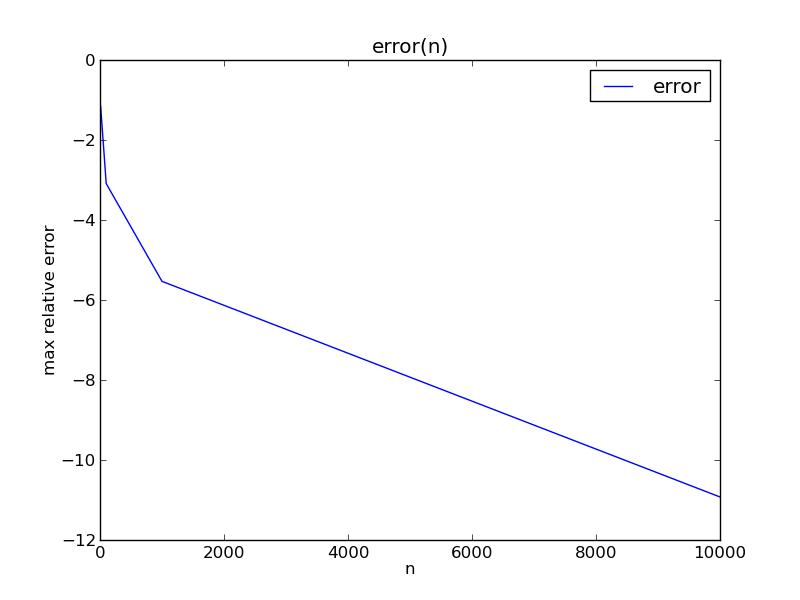
\includegraphics[scale=0.5]{max_error.jpg}}
  \end{center}
  \caption{\textit{plot of max relative error for n = 10, 100, 1000, 10000}}
  \label{fig:edge}
\end{figure}

In this plot we se that the relative error gets smaller end smaller for higher values of n. this is what we would expect as we
get higher numerical precision. 

\subsection*{part d)}

In this section we are going to compare the algorithm to a standard algoritm by using armadillo's lu() and solve() functions.
I am first going to make a plot of the time used to compute with my algoritm vs the time used to compute by LU decomposition
and solving in armadillo.

\begin{figure}[H]
  \begin{center}
    \subfigure[N = 10]{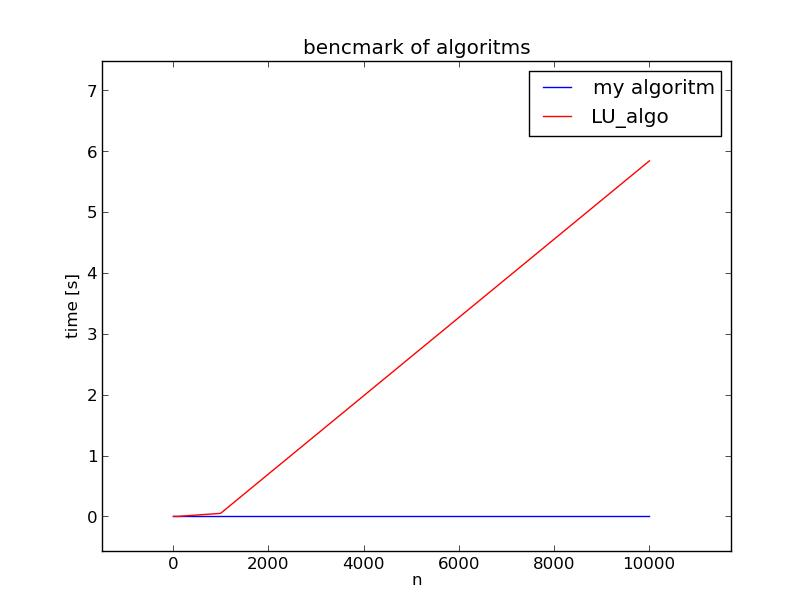
\includegraphics[scale=0.5]{benchmark.jpg}}
  \end{center}
  \caption{\textit{plot benchmark times for the two different methods of solving}}
  \label{fig:edge}
\end{figure}

The numbers i got for mu algorithm where all $0.0$ i tried to figurre out how to get a higher precision in the timer with no luck.
But the point still stands here. We can see that my algorithm solves in basically the same time for all values of n. 
While the Armadillo version seems to shoot in the ``sky'' exponentially. This is expected though scince the Armadillo algorithm
typically uses $n^2 + n^3$ flops while mine uses $8(n-1)$ flops and therefore is much more effective.
 
\newpage

\section*{Attachments}

\textbf{Attachment 1: C++ main program}\newline

\lstinputlisting[language=C++]{main.cpp}
\newpage

\textbf{Attachment 2: python script for ploting values from a file}\newline

\lstinputlisting[language=Python]{plot.py}
\newpage
\textbf{Attachment 3: python script for computing and ploting error}\newline

\lstinputlisting[language=Python]{error.py}
\newpage
\textbf{Attachment 4: python script for ploting benchmark times}\newline

\lstinputlisting[language=Python]{bench.py}


%``i ain't no damn scientist!''
\end{document}








